% This is the Reed College LaTeX thesis template. Most of the work
% for the document class was done by Sam Noble (SN), as well as this
% template. Later comments etc. by Ben Salzberg (BTS). Additional
% restructuring and APA support by Jess Youngberg (JY).
% Your comments and suggestions are more than welcome; please email
% them to cus@reed.edu
%
% See http://web.reed.edu/cis/help/latex.html for help. There are a
% great bunch of help pages there, with notes on
% getting started, bibtex, etc. Go there and read it if you're not
% already familiar with LaTeX.
%
% Any line that starts with a percent symbol is a comment.
% They won't show up in the document, and are useful for notes
% to yourself and explaining commands.
% Commenting also removes a line from the document;
% very handy for troubleshooting problems. -BTS

% As far as I know, this follows the requirements laid out in
% the 2002-2003 Senior Handbook. Ask a librarian to check the
% document before binding. -SN

%%
%% Preamble
%%
% \documentclass{<something>} must begin each LaTeX document
\documentclass[12pt,twoside]{reedthesis}
% Packages are extensions to the basic LaTeX functions. Whatever you
% want to typeset, there is probably a package out there for it.
% Chemistry (chemtex), screenplays, you name it.
% Check out CTAN to see: http://www.ctan.org/
%%
\usepackage{graphicx,latexsym}
\usepackage[french]{babel} 
\usepackage{amsmath}
\usepackage{amssymb,amsthm}
\usepackage{xcolor}
\usepackage{eso-pic}
\usepackage{longtable,booktabs,setspace}
\usepackage{chemarr} %% Useful for one reaction arrow, useless if you're not a chem major
\usepackage[hyphens]{url}
\usepackage{tikz}
\usetikzlibrary{calc}
\newcommand\HRule{\rule{\textwidth}{1pt}}
% Added by CII
\usepackage{hyperref}
\usepackage{lmodern}
\usepackage{float}
\floatplacement{figure}{H}
% End of CII addition
\usepackage{rotating}

% Next line commented out by CII
%%% \usepackage{natbib}
% Comment out the natbib line above and uncomment the following two lines to use the new
% biblatex-chicago style, for Chicago A. Also make some changes at the end where the
% bibliography is included.
%\usepackage{biblatex-chicago}
%\bibliography{thesis}


% Added by CII (Thanks, Hadley!)
% Use ref for internal links
\renewcommand{\hyperref}[2][???]{\autoref{#1}}
\def\chapterautorefname{Chapter}
\def\sectionautorefname{Section}
\def\subsectionautorefname{Subsection}
% End of CII addition

% Added by CII
\usepackage{caption}
\captionsetup{width=5in}
% End of CII addition

% \usepackage{times} % other fonts are available like times, bookman, charter, palatino


% To pass between YAML and LaTeX the dollar signs are added by CII
\title{THÈSE}
\author{Keurcien LUU}
\labo{Techniques de l'Ingénierie Médicale et de la Complexité - Informatique,
Mathématiques et Applications de Grenoble (TIMC-IMAG)}
% The month and year that you submit your FINAL draft TO THE LIBRARY (May or December)
\date{31 octobre 2017}
\division{Mathematics and Natural Sciences}
\advisor{Michael BLUM}
%If you have two advisors for some reason, you can use the following
% Uncommented out by CII
% End of CII addition

%%% Remember to use the correct department!
\department{Ingénierie de la Santé, de la Cognition et Environnement (EDISCE)}
% if you're writing a thesis in an interdisciplinary major,
% uncomment the line below and change the text as appropriate.
% check the Senior Handbook if unsure.
%\thedivisionof{The Established Interdisciplinary Committee for}
% if you want the approval page to say "Approved for the Committee",
% uncomment the next line
%\approvedforthe{Committee}

% Added by CII
%%% Copied from knitr
%% maxwidth is the original width if it's less than linewidth
%% otherwise use linewidth (to make sure the graphics do not exceed the margin)
\makeatletter
\def\maxwidth{ %
  \ifdim\Gin@nat@width>\linewidth
    \linewidth
  \else
    \Gin@nat@width
  \fi
}
\makeatother

\renewcommand{\contentsname}{Table of Contents}
% End of CII addition

\setlength{\parskip}{0pt}

% Added by CII

\providecommand{\tightlist}{%
  \setlength{\itemsep}{0pt}\setlength{\parskip}{0pt}}

\Acknowledgements{
Je tiens à remercier mes collègues Kevin Caye, Thomas Dias-Alves, Thomas
Karaouzène et Florian Privé, avec qui j'ai partagé ces trois années de
thèse et de qui j'ai beaucoup appris.
}

\Dedication{

}

\Preface{
This is an example of a thesis setup to use the reed thesis document
class (for LaTeX) and the R bookdown package, in general.
}

\Abstract{
The preface pretty much says it all. \par  Second paragraph of abstract
starts here.
}

% End of CII addition
%%
%% End Preamble
%%
%

\usepackage{amsthm}
\newtheorem{theorem}{Theorem}[section]
\newtheorem{lemma}{Lemma}[section]
\theoremstyle{definition}
\newtheorem{definition}{Definition}[section]
\newtheorem{corollary}{Corollary}[section]
\newtheorem{proposition}{Proposition}[section]
\theoremstyle{definition}
\newtheorem{example}{Example}[section]
\theoremstyle{remark}
\newtheorem*{remark}{Remark}
\begin{document}

% Everything below added by CII
      \maketitle
  
  \frontmatter % this stuff will be roman-numbered
  \pagestyle{empty} % this removes page numbers from the frontmatter

      \begin{acknowledgements}
      Je tiens à remercier mes collègues Kevin Caye, Thomas Dias-Alves, Thomas
      Karaouzène et Florian Privé, avec qui j'ai partagé ces trois années de
      thèse et de qui j'ai beaucoup appris.
    \end{acknowledgements}
  
      \begin{preface}
      This is an example of a thesis setup to use the reed thesis document
      class (for LaTeX) and the R bookdown package, in general.
    \end{preface}
  
      \hypersetup{linkcolor=black}
    \setcounter{tocdepth}{2}
    \tableofcontents
  
      \listoftables
  
      \listoffigures
  
      \begin{abstract}
      The preface pretty much says it all. \par  Second paragraph of abstract
      starts here.
    \end{abstract}
  
  
  \mainmatter % here the regular arabic numbering starts
  \pagestyle{fancyplain} % turns page numbering back on

  \chapter{thesis\_pdf\_updt: default}\label{thesis_pdf_updt-default}
  
  \chapter{État de l'art}\label{etat-de-lart}
  
  \chapter{Adaptation locale}\label{adaptation-locale}
  
  \chapter{Introgression adaptative}\label{introgression-adaptative}
  
  \section{Qu'est-ce que l'introgression
  ?}\label{quest-ce-que-lintrogression}
  
  Avant de s'intéresser à la notion d'introgression, intéressons-nous
  d'abord à celle d'hybridation. L'hybridation peut être définie comme la
  reproduction entre deux individus appartenant à deux espèces ou à deux
  populations différentes. Cette définition nous amène à nous poser deux
  questions. La première, relative à la notion d'espèce, est souvent
  sujette à controverse. La seconde concerne quant à elle la désignation
  de populations différentes. Qu'est-ce qui fait que deux groupes
  d'individus sont différents ? Harrison suggère en 1990 que deux
  individus issus de populations différentes doivent chacun posséder des
  traits héritables qui les différencient (Harrison \& others, 1990).
  
  Nous parlons d'introgression lorsqu'un certain nombre de gènes est
  transféré d'une population à une autre.
  
  \section{Coefficients de métissage globaux et
  locaux}\label{coefficients-de-metissage-globaux-et-locaux}
  
  Étant données des populations ancestrales, il est possible d'estimer
  pour un individu donné, la proportion de son génôme provenant de chacune
  des populations ancestrales. Ces proportions sont connues plus
  communément sous le nom de \emph{coefficients de métissage globaux}. De
  nombreux logiciels existent pour l'estimation de ces coefficients :
  STRUCTURE, ADMIXTURE (Alexander, 2009), LEA (Frichot, 2015), tess3r
  (Caye, 2016). En complément à cette information globale, il peut être
  intéressant de déterminer sur des portions plus petites du génôme, de la
  même manière que dans le cas global, les proportions venant de telle ou
  telle population ancestrale pour chacune de ces portions. Nous parlons
  dans ce cas de \emph{coefficients de métissage locaux}. Encore une fois,
  plusieurs logiciels ont été proposés dans le but d'estimer ces
  coefficients : Hapmix (Price, 2009), EILA (Yang, 2013), LAMP (Thornton,
  2014), loter ou encore RFmix (Maples, 2013).
  
  \section{Introgression}\label{introgression}
  
  L'introgression peut être détectée de différentes façons. Une première
  approche consiste à utiliser les \emph{coefficients de métissage
  locaux}. Les méthodes mentionnées plus haut estiment ces coefficients
  pour chaque individu, permettant de calculer à partir de ceux-ci des
  coefficients de métissage locaux pour chaque population.
  
  \section{Lien entre Analyse en Composantes Principales et métissage
  global.}\label{lien-entre-analyse-en-composantes-principales-et-metissage-global.}
  
  L'un des premiers articles à établir un lien entre l'ACP et les
  coefficients de métissage global fut sur l'interprétation généalogique
  de l'ACP de Gil McVean (McVean, 2009):
  
  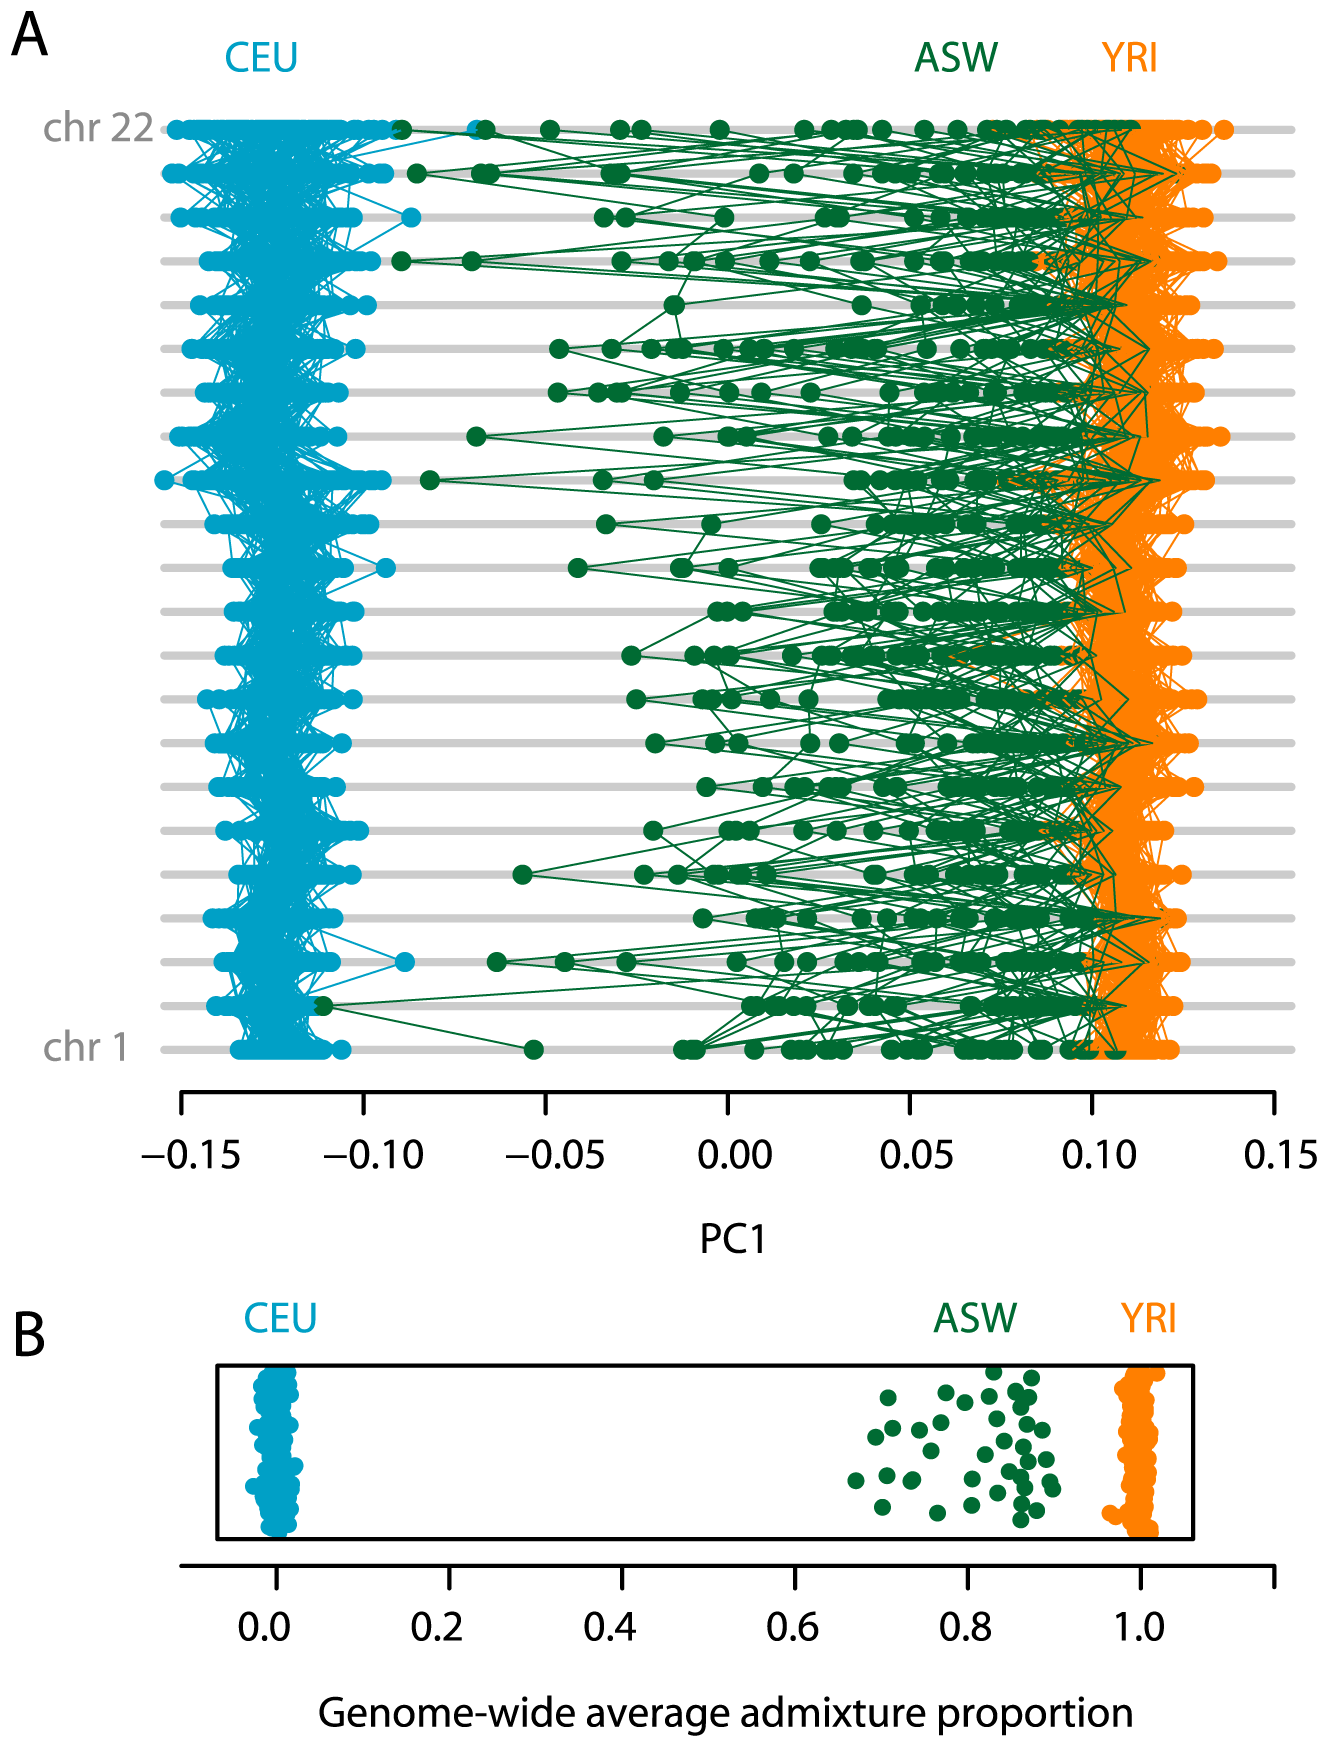
\includegraphics[width=250pt]{figure/mcvean.png}
  
  Pour chacun des 22 chromosomes,
  
  \section{Analyse en Composantes Principales
  locale}\label{analyse-en-composantes-principales-locale}
  
  Notant \(p\) le nombre de marqueurs génétiques, \(i\) un entier compris
  entre \(1\) et \(p\), et \(x_i\) la position génétique (en Morgans) ou
  la position physique (en paires de bases) du \(i\)-ème marqueur
  génétique. Nous définissons pour cet entier \(i\) la fenêtre \(W_i^T\)
  de taille \(T\) et centrée en \(i\) :
  
  \[W_i^T = \{ j \in [|1, p|], |x_i - x_j| \leq T/2 \}\]
  
  \section{Sensibilité à l'imputation des données
  manquantes}\label{sensibilite-a-limputation-des-donnees-manquantes}
  
  \section{Simulations}\label{simulations}
  
  \subsection{Données de peupliers}\label{donnees-de-peupliers}
  
  Le premier jeu de données est issu d'une étude d'introgression
  adaptative chez les peupliers d'Amérique du Nord (Suarez-Gonzalez,
  2016). La simulation d'haplotypes d'individus admixés est effectuée à
  partir des deux populations ancestrales qui y sont présentes. La
  première, \emph{Populus Balsamifera}, est une espèce de peupliers qui
  peuple le nord du continent nord-américain, d'Est en Ouest, et se trouve
  exposée à des conditions climatiques peu clémentes. La seconde,
  \emph{Populus Trichocarpa}, est principalement localisée en Californie,
  et bénéficie d'un climat continental.
  
  Chacune des simulations est constituée de \(50\) haplotypes de la souche
  continentale, de \(50\) haplotyêpes de la souche boréale, ainsi que de
  \(50\) haplotypes d'individus hybrides générés à partir des haplotypes
  ancestraux. Ces haplotypes ancestraux ont été estimés à l'aide du
  logiciel Beagle. 'A partir des positions en paires de base, une carte de
  recombinaison génétique est générée en utilisant le taux de
  recombinaison moyen chez le peuplier. Le taux de recombinaison, noté
  \(\tau_r\), correspond au nombre moyen de paires de bases à parcourir
  pour qu'ait lieu un épisode de recombinaison génétique, \emph{i.e.},
  notant \(L\) la longueur du chromosome en Morgans (\(M\)), et \(N_{bp}\)
  le nombre de paires de bases le constituant, le taux de recombinaison
  génétique pour ce chromosome est donné par la relation:
  
  \[\tau_r = \frac{L}{N_{bp}}\]
  
  Dans ce scénario, les simulations ont été produites en utilisant un taux
  de recombinaison génétique moyen \(\tau_r\) de \(0.05\) centiMorgans par
  million de paire de bases, correspondant à la valeur utilisée par les
  auteurs de l'étude avec le logiciel RASPberry
  (\textit{Recombination via Ancestry Switch Probability}). A partir de la
  donnée de la position physique en paires de bases ainsi que du taux de
  recombinaison moyen, nous générons une carte de recombinaison génétique
  adaptée à nos simulations.
  
  \subsection{Génération aléatoire d'individus
  hybrides}\label{generation-aleatoire-dindividus-hybrides}
  
  Pour simuler un individu métissé, il est d'abord nécessaire de simuler
  l'emplacement des évènements de recombinaison. Pour ce faire, nous
  utilisons le modèle décrit dans (Price, 2009), en parcourant
  
  \begin{figure}
  
  {\centering 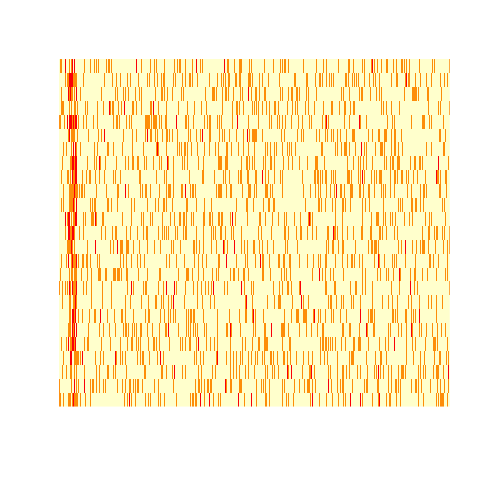
\includegraphics[width=400px,height=200px]{figure/ancestry_heatmap_lambda_0001} 
  
  }
  
  \caption{$\lambda = 0.001$}\label{fig:lambda0001}
  \end{figure}\begin{figure}
  
  {\centering 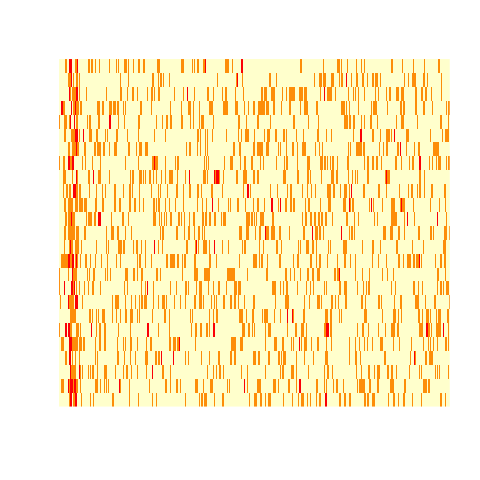
\includegraphics[width=400px,height=200px]{figure/ancestry_heatmap_lambda_001} 
  
  }
  
  \caption{$\lambda = 0.01$}\label{fig:lambda001}
  \end{figure}\begin{figure}
  
  {\centering 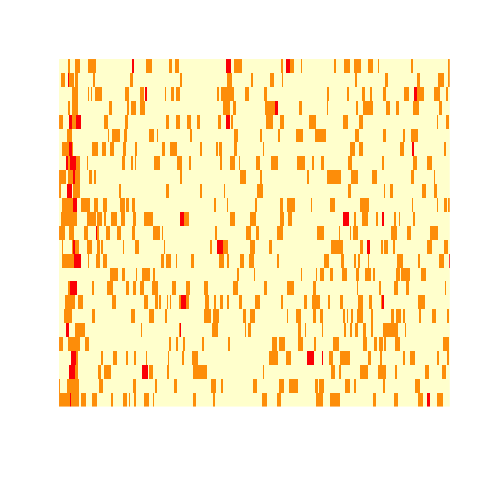
\includegraphics[width=400px,height=200px]{figure/ancestry_heatmap_lambda_01} 
  
  }
  
  \caption{$\lambda = 0.1$}\label{fig:lambda01}
  \end{figure}
  
  \begin{Shaded}
  \begin{Highlighting}[]
  \NormalTok{path <-}\StringTok{ "~/Documents/thesis/git/simulations/introgression/"}
  \NormalTok{output.name <-}\StringTok{ "populus"}
  \NormalTok{recombinationRate <-}\StringTok{ }\FloatTok{0.05} \CommentTok{# in Morgans per Megabase}
  \NormalTok{nSNP <-}\StringTok{ }\DecValTok{50000}
  \NormalTok{ancstrl}\FloatTok{.1} \NormalTok{<-}\StringTok{ }\DecValTok{1}
  \NormalTok{ancstrl}\FloatTok{.2} \NormalTok{<-}\StringTok{ }\DecValTok{3}
  \NormalTok{hyb <-}\StringTok{ }\DecValTok{4}
  \NormalTok{intro.size <-}\StringTok{ }\DecValTok{500}
  \NormalTok{global.ancestry <-}\StringTok{ }\FloatTok{0.1}
  \NormalTok{inverted.ancestry <-}\StringTok{ }\FloatTok{0.5}
  
  \NormalTok{info.map <-}\StringTok{ }\KeywordTok{as.matrix}\NormalTok{(data.table::}\KeywordTok{fread}\NormalTok{(}\KeywordTok{paste0}\NormalTok{(path, output.name, }\StringTok{".map"}\NormalTok{), }
                                          \DataTypeTok{data.table =} \OtherTok{FALSE}\NormalTok{))}
  \NormalTok{H1 <-}\StringTok{ }\KeywordTok{as.matrix}\NormalTok{(data.table::}\KeywordTok{fread}\NormalTok{(}\KeywordTok{paste0}\NormalTok{(path, output.name, }\StringTok{"_H1"}\NormalTok{), }
                                    \DataTypeTok{data.table =} \OtherTok{FALSE}\NormalTok{))}
  \NormalTok{H2 <-}\StringTok{ }\KeywordTok{as.matrix}\NormalTok{(data.table::}\KeywordTok{fread}\NormalTok{(}\KeywordTok{paste0}\NormalTok{(path, output.name, }\StringTok{"_H2"}\NormalTok{), }
                                    \DataTypeTok{data.table =} \OtherTok{FALSE}\NormalTok{))}
  \NormalTok{n.hyb <-}\StringTok{ }\KeywordTok{ncol}\NormalTok{(H1) /}\StringTok{ }\DecValTok{2} 
  
  \NormalTok{### Introgression region}
  \NormalTok{idx <-}\StringTok{ }\KeywordTok{sample}\NormalTok{(}\DecValTok{1}\NormalTok{:nSNP, }\DataTypeTok{size =} \DecValTok{1}\NormalTok{)}
  \NormalTok{beg.reg <-}\StringTok{ }\KeywordTok{max}\NormalTok{(}\DecValTok{1}\NormalTok{, idx -}\StringTok{ }\NormalTok{intro.size)}
  \NormalTok{end.reg <-}\StringTok{ }\KeywordTok{min}\NormalTok{(nSNP, idx +}\StringTok{ }\NormalTok{intro.size)}
  \NormalTok{intro.reg <-}\StringTok{ }\NormalTok{beg.reg:end.reg}
  \end{Highlighting}
  \end{Shaded}
  
  \newpage
  
  \newpage
  
  \subsection{Résultats de la comparaison des
  logiciels}\label{resultats-de-la-comparaison-des-logiciels}
  
  \begin{Shaded}
  \begin{Highlighting}[]
  \KeywordTok{setwd}\NormalTok{(}\StringTok{"~/Documents/thesis/git/simulations/introgression/"}\NormalTok{)}
  \NormalTok{output.name <-}\StringTok{ "populus"}
  \NormalTok{recombinationRate <-}\StringTok{ }\FloatTok{0.05} \CommentTok{# in Morgans per Megabase}
  \NormalTok{nSNP <-}\StringTok{ }\DecValTok{50000}
  \NormalTok{ancstrl}\FloatTok{.1} \NormalTok{<-}\StringTok{ }\DecValTok{1}
  \NormalTok{ancstrl}\FloatTok{.2} \NormalTok{<-}\StringTok{ }\DecValTok{3}
  \NormalTok{hyb <-}\StringTok{ }\DecValTok{4}
  \NormalTok{intro.size <-}\StringTok{ }\DecValTok{500}
  \NormalTok{global.ancestry <-}\StringTok{ }\FloatTok{0.1}
  \NormalTok{inverted.ancestry <-}\StringTok{ }\FloatTok{0.5}
  \NormalTok{N <-}\StringTok{ }\DecValTok{10}
  \NormalTok{pop <-}\StringTok{ }\KeywordTok{c}\NormalTok{(}\KeywordTok{rep}\NormalTok{(ancstrl}\FloatTok{.1}\NormalTok{, }\KeywordTok{ncol}\NormalTok{(H1) /}\StringTok{ }\DecValTok{2}\NormalTok{), }
           \KeywordTok{rep}\NormalTok{(ancstrl}\FloatTok{.2}\NormalTok{, }\KeywordTok{ncol}\NormalTok{(H2) /}\StringTok{ }\DecValTok{2}\NormalTok{), }
           \KeywordTok{rep}\NormalTok{(}\DecValTok{4}\NormalTok{, n.hyb))}
  \NormalTok{results <-}\StringTok{ }\KeywordTok{data.frame}\NormalTok{(}\DataTypeTok{Software =} \KeywordTok{c}\NormalTok{(}\StringTok{"pcadapt"}\NormalTok{, }\StringTok{"eila"}\NormalTok{, }\StringTok{"RFMix"}\NormalTok{), }\DataTypeTok{Power =} \KeywordTok{c}\NormalTok{(}\DecValTok{0}\NormalTok{, }\DecValTok{0}\NormalTok{, }\DecValTok{0}\NormalTok{), }\DataTypeTok{FDR =} \KeywordTok{c}\NormalTok{(}\DecValTok{0}\NormalTok{, }\DecValTok{0}\NormalTok{, }\DecValTok{0}\NormalTok{))}
  \NormalTok{info.map <-}\StringTok{ }\KeywordTok{as.matrix}\NormalTok{(data.table::}\KeywordTok{fread}\NormalTok{(}\KeywordTok{paste0}\NormalTok{(path, output.name, }\StringTok{".map"}\NormalTok{), }
                                          \DataTypeTok{data.table =} \OtherTok{FALSE}\NormalTok{))}
  
  \NormalTok{compute.fdr =}\StringTok{ }\NormalTok{function(list, ground.truth)\{}
    \NormalTok{if (}\KeywordTok{length}\NormalTok{(list) ==}\StringTok{ }\DecValTok{0}\NormalTok{)\{}
      \NormalTok{x <-}\StringTok{ }\DecValTok{0}
    \NormalTok{\} else \{}
      \NormalTok{x <-}\StringTok{ }\KeywordTok{sum}\NormalTok{(!(list %in%}\StringTok{ }\NormalTok{ground.truth)) /}\StringTok{ }\KeywordTok{length}\NormalTok{(list)}
    \NormalTok{\}}
    \KeywordTok{return}\NormalTok{(x)}
  \NormalTok{\}}
  
  \NormalTok{compute.power =}\StringTok{ }\NormalTok{function(list, ground.truth)\{}
    \NormalTok{if (}\KeywordTok{length}\NormalTok{(ground.truth) ==}\StringTok{ }\DecValTok{0}\NormalTok{)\{}
      \KeywordTok{warning}\NormalTok{(}\StringTok{"The list of true positives is empty."}\NormalTok{)}
    \NormalTok{\} else \{}
      \NormalTok{x <-}\StringTok{ }\KeywordTok{sum}\NormalTok{(list %in%}\StringTok{ }\NormalTok{ground.truth) /}\StringTok{ }\KeywordTok{length}\NormalTok{(ground.truth)}
    \NormalTok{\}}
    \KeywordTok{return}\NormalTok{(x)}
  \NormalTok{\}}
  
  \NormalTok{for (n.simu in }\DecValTok{21}\NormalTok{:}\DecValTok{30}\NormalTok{)\{}
    \NormalTok{dir.name <-}\StringTok{ }\KeywordTok{paste0}\NormalTok{(}\StringTok{"RFMix_v1.5.4/simu"}\NormalTok{, n.simu, }\StringTok{"/"}\NormalTok{)}
    
    \NormalTok{input.pcadapt <-}\StringTok{ }\KeywordTok{as.matrix}\NormalTok{(data.table::}\KeywordTok{fread}\NormalTok{(}\KeywordTok{paste0}\NormalTok{(dir.name, }\StringTok{"simu.pcadapt"}\NormalTok{), }\DataTypeTok{data.table =} \OtherTok{FALSE}\NormalTok{))}
    \NormalTok{input.eila <-}\StringTok{ }\NormalTok{simulate::}\KeywordTok{eila_from_pcadapt}\NormalTok{(input.pcadapt, pop, }\DataTypeTok{anc1 =} \NormalTok{ancstrl}\FloatTok{.1}\NormalTok{, }\DataTypeTok{anc2 =} \NormalTok{ancstrl}\FloatTok{.2}\NormalTok{, }\DataTypeTok{admixed =} \NormalTok{hyb, }\DataTypeTok{position =} \NormalTok{info.map[, }\DecValTok{2}\NormalTok{])}
    \NormalTok{param <-}\StringTok{ }\KeywordTok{read.table}\NormalTok{(}\KeywordTok{paste0}\NormalTok{(dir.name, }\StringTok{"/parameters.txt"}\NormalTok{))}
    \NormalTok{gt <-}\StringTok{ }\NormalTok{(param$begin):(param$end)}
    
    \NormalTok{### run pcadapt}
    \NormalTok{wsize <-}\StringTok{ }\DecValTok{1000}
    \NormalTok{mmaf <-}\StringTok{ }\FloatTok{0.01}
    \NormalTok{nomap <-}\StringTok{ }\DecValTok{1}\NormalTok{:nSNP}
    \NormalTok{maf <-}\StringTok{ }\NormalTok{pcadapt::}\KeywordTok{cmpt_minor_af}\NormalTok{(input.pcadapt, }\DecValTok{2}\NormalTok{)}
    \NormalTok{proxy.map <-}\StringTok{ }\NormalTok{info.map[}\DecValTok{1}\NormalTok{:nSNP]}
    \NormalTok{filtered.map <-}\StringTok{ }\NormalTok{nomap[maf >=}\StringTok{ }\NormalTok{mmaf]}
    \NormalTok{stat.pcadapt <-}\StringTok{ }\NormalTok{pcadapt::}\KeywordTok{scan.intro}\NormalTok{(input.pcadapt, }\DataTypeTok{K =} \DecValTok{1}\NormalTok{, }\DataTypeTok{pop =} \NormalTok{pop, }
                               \DataTypeTok{ancstrl.1 =} \NormalTok{ancstrl}\FloatTok{.2}\NormalTok{, }
                               \DataTypeTok{ancstrl.2 =} \NormalTok{ancstrl}\FloatTok{.1}\NormalTok{,}
                               \DataTypeTok{admxd =} \NormalTok{hyb,}
                               \DataTypeTok{min.maf =} \NormalTok{mmaf,}
                               \DataTypeTok{window.size =} \NormalTok{wsize,}
                               \DataTypeTok{ploidy =} \DecValTok{2}\NormalTok{,}
                               \DataTypeTok{side =} \StringTok{"middle"}\NormalTok{,}
                               \DataTypeTok{map =} \NormalTok{nomap)}
    
    \NormalTok{### run eila }
    \NormalTok{obj.eila <-}\StringTok{ }\NormalTok{EILA::}\KeywordTok{eila}\NormalTok{(}\DataTypeTok{admixed =} \NormalTok{input.eila$admixed, }\DataTypeTok{anc1 =} \NormalTok{input.eila$anc1,}
                           \DataTypeTok{anc2 =} \NormalTok{input.eila$anc2, }\DataTypeTok{position =} \NormalTok{info.map[, }\DecValTok{1}\NormalTok{], }\DataTypeTok{lambda =} \FloatTok{0.1}\NormalTok{)}
    \NormalTok{loc.anc.eila <-}\StringTok{ }\NormalTok{simulate::}\KeywordTok{haplo_to_ancestry}\NormalTok{(obj.eila$local.ancestry, }\DecValTok{1}\NormalTok{)}
    
    \NormalTok{### run rfmix}
    \NormalTok{allele <-}\StringTok{ }\KeywordTok{paste0}\NormalTok{(}\StringTok{"./simu"}\NormalTok{, n.simu, }\StringTok{"/rfmix_alleles.txt"}\NormalTok{)}
    \NormalTok{classes <-}\StringTok{ }\KeywordTok{paste0}\NormalTok{(}\StringTok{"./simu"}\NormalTok{, n.simu, }\StringTok{"/rfmix_classes.txt"}\NormalTok{)}
    \NormalTok{markerLocation <-}\StringTok{  }\KeywordTok{paste0}\NormalTok{(}\StringTok{"./simu"}\NormalTok{, n.simu, }\StringTok{"/rfmix_markerLocation.txt"}\NormalTok{)}
    \NormalTok{output <-}\StringTok{ }\KeywordTok{paste0}\NormalTok{(}\StringTok{"simu"}\NormalTok{, n.simu, }\StringTok{"/output_simu"}\NormalTok{, n.simu)}
    \NormalTok{window.rfmix <-}\StringTok{ }\FloatTok{0.00002}
    \NormalTok{command <-}\StringTok{ }\KeywordTok{paste}\NormalTok{(}\StringTok{"python2.7 RunRFMix.py PopPhased"}\NormalTok{, allele,  classes,  markerLocation, }\StringTok{"-w"}\NormalTok{, window.rfmix, }\StringTok{"-o"}\NormalTok{, output)}
    \KeywordTok{setwd}\NormalTok{(}\StringTok{"~/Documents/thesis/git/simulations/introgression/RFMix_v1.5.4/"}\NormalTok{)}
    \KeywordTok{system}\NormalTok{(}\DataTypeTok{command =} \NormalTok{command)}
    \KeywordTok{setwd}\NormalTok{(}\StringTok{"~/Documents/thesis/git/simulations/introgression/"}\NormalTok{)}
    \NormalTok{aux.rfmix <-}\StringTok{ }\NormalTok{simulate::}\KeywordTok{rfmix.local.ancestry}\NormalTok{(}\KeywordTok{paste0}\NormalTok{(}\StringTok{"RFMix_v1.5.4/simu"}\NormalTok{, n.simu, }\StringTok{"/output_simu"}\NormalTok{, n.simu, }\StringTok{".0.Viterbi.txt"}\NormalTok{))}
    \NormalTok{loc.anc.rfmix <-}\StringTok{ }\NormalTok{simulate::}\KeywordTok{haplo_to_ancestry}\NormalTok{(aux.rfmix, }\DecValTok{1}\NormalTok{)}
    
    \NormalTok{### FDR}
    \NormalTok{interp <-}\StringTok{ }\KeywordTok{approx}\NormalTok{(filtered.map, stat.pcadapt[[}\DecValTok{1}\NormalTok{]], }\DecValTok{1}\NormalTok{:nSNP)}
    \NormalTok{sd.pcadapt <-}\StringTok{ }\KeywordTok{sd}\NormalTok{(interp$y, }\DataTypeTok{na.rm =} \OtherTok{TRUE}\NormalTok{)}
    \NormalTok{list.pcadapt <-}\StringTok{ }\KeywordTok{which}\NormalTok{(interp$y >}\StringTok{ }\DecValTok{3}\NormalTok{)}
    \NormalTok{results[}\DecValTok{1}\NormalTok{, }\DecValTok{3}\NormalTok{] <-}\StringTok{ }\NormalTok{results[}\DecValTok{1}\NormalTok{, }\DecValTok{3}\NormalTok{] +}\StringTok{ }\KeywordTok{compute.fdr}\NormalTok{(list.pcadapt, gt) /}\StringTok{ }\NormalTok{N}
    \NormalTok{results[}\DecValTok{1}\NormalTok{, }\DecValTok{2}\NormalTok{] <-}\StringTok{ }\NormalTok{results[}\DecValTok{1}\NormalTok{, }\DecValTok{2}\NormalTok{] +}\StringTok{ }\KeywordTok{compute.power}\NormalTok{(list.pcadapt, gt) /}\StringTok{ }\NormalTok{N}
    
    \NormalTok{sd.eila <-}\StringTok{ }\KeywordTok{sd}\NormalTok{(loc.anc.eila, }\DataTypeTok{na.rm =} \OtherTok{TRUE}\NormalTok{)}
    \NormalTok{stat.eila <-}\StringTok{ }\NormalTok{(loc.anc.eila -}\StringTok{ }\KeywordTok{mean}\NormalTok{(loc.anc.eila)) /}\StringTok{ }\NormalTok{sd.eila}
    \NormalTok{list.eila <-}\StringTok{ }\KeywordTok{which}\NormalTok{(stat.eila >}\StringTok{ }\DecValTok{3}\NormalTok{)}
    \NormalTok{results[}\DecValTok{2}\NormalTok{, }\DecValTok{3}\NormalTok{] <-}\StringTok{ }\NormalTok{results[}\DecValTok{2}\NormalTok{, }\DecValTok{3}\NormalTok{] +}\StringTok{ }\KeywordTok{compute.fdr}\NormalTok{(list.eila, gt) /}\StringTok{ }\NormalTok{N}
    \NormalTok{results[}\DecValTok{2}\NormalTok{, }\DecValTok{2}\NormalTok{] <-}\StringTok{ }\NormalTok{results[}\DecValTok{2}\NormalTok{, }\DecValTok{2}\NormalTok{] +}\StringTok{ }\KeywordTok{compute.power}\NormalTok{(list.eila, gt) /}\StringTok{ }\NormalTok{N}
    
    \NormalTok{sd.rfmix <-}\StringTok{ }\KeywordTok{sd}\NormalTok{(loc.anc.rfmix, }\DataTypeTok{na.rm =} \OtherTok{TRUE}\NormalTok{)}
    \NormalTok{stat.rfmix <-}\StringTok{ }\NormalTok{(loc.anc.rfmix -}\StringTok{ }\KeywordTok{mean}\NormalTok{(loc.anc.rfmix)) /}\StringTok{ }\NormalTok{sd.rfmix}
    \NormalTok{list.rfmix <-}\StringTok{ }\KeywordTok{which}\NormalTok{(stat.rfmix >}\StringTok{ }\DecValTok{3}\NormalTok{)}
    \NormalTok{results[}\DecValTok{3}\NormalTok{, }\DecValTok{3}\NormalTok{] <-}\StringTok{ }\NormalTok{results[}\DecValTok{3}\NormalTok{, }\DecValTok{3}\NormalTok{] +}\StringTok{ }\KeywordTok{compute.fdr}\NormalTok{(list.rfmix, gt) /}\StringTok{ }\NormalTok{N}
    \NormalTok{results[}\DecValTok{3}\NormalTok{, }\DecValTok{2}\NormalTok{] <-}\StringTok{ }\NormalTok{results[}\DecValTok{3}\NormalTok{, }\DecValTok{2}\NormalTok{] +}\StringTok{ }\KeywordTok{compute.power}\NormalTok{(list.rfmix, gt) /}\StringTok{ }\NormalTok{N}
  \NormalTok{\}}
  
  
  \NormalTok{ggres <-}\StringTok{ }\KeywordTok{data.frame}\NormalTok{(}\DataTypeTok{Software =} \KeywordTok{rep}\NormalTok{(}\KeywordTok{c}\NormalTok{(}\StringTok{"pcadapt"}\NormalTok{, }\StringTok{"eila"}\NormalTok{, }\StringTok{"RFMix"}\NormalTok{), }\DecValTok{2}\NormalTok{), }\DataTypeTok{Stat =} \KeywordTok{rep}\NormalTok{(}\DecValTok{0}\NormalTok{, }\DecValTok{6}\NormalTok{), }\DataTypeTok{Type =} \KeywordTok{c}\NormalTok{(}\KeywordTok{rep}\NormalTok{(}\StringTok{"Power"}\NormalTok{, }\DecValTok{3}\NormalTok{), }\KeywordTok{rep}\NormalTok{(}\StringTok{"FDR"}\NormalTok{, }\DecValTok{3}\NormalTok{)), }
                      \DataTypeTok{Percent =} \KeywordTok{rep}\NormalTok{(}\DecValTok{0}\NormalTok{, }\DecValTok{6}\NormalTok{))}
  \NormalTok{ggres$Stat[}\DecValTok{1}\NormalTok{:}\DecValTok{3}\NormalTok{] <-}\StringTok{ }\NormalTok{results$Power *}\StringTok{ }\DecValTok{100}
  \NormalTok{ggres$Stat[}\DecValTok{4}\NormalTok{:}\DecValTok{6}\NormalTok{] <-}\StringTok{ }\NormalTok{results$FDR *}\StringTok{ }\DecValTok{100}
  \NormalTok{ggres$Percent <-}\StringTok{ }\KeywordTok{as.numeric}\NormalTok{(}\KeywordTok{format}\NormalTok{(ggres$Stat, }\DataTypeTok{digits =} \DecValTok{2}\NormalTok{))}
  \NormalTok{p0 <-}\StringTok{ }\KeywordTok{ggplot}\NormalTok{(ggres, }\KeywordTok{aes}\NormalTok{(}\DataTypeTok{x =} \NormalTok{Software, }\DataTypeTok{y =} \NormalTok{Stat, }\DataTypeTok{fill =} \KeywordTok{as.factor}\NormalTok{(Type)))}
  \NormalTok{p0 <-}\StringTok{ }\NormalTok{p0 +}\StringTok{ }\KeywordTok{ggtitle}\NormalTok{(}\KeywordTok{expression}\NormalTok{(lambda ==}\StringTok{ }\DecValTok{1}\NormalTok{)) +}\StringTok{ }\KeywordTok{ylab}\NormalTok{(}\StringTok{""}\NormalTok{)}
  \NormalTok{p0 <-}\StringTok{ }\NormalTok{p0 +}\StringTok{ }\KeywordTok{geom_bar}\NormalTok{(}\DataTypeTok{stat =} \StringTok{"identity"}\NormalTok{, }\DataTypeTok{position =} \KeywordTok{position_dodge}\NormalTok{(}\DataTypeTok{width =} \FloatTok{0.9}\NormalTok{))}
  \NormalTok{p0 <-}\StringTok{ }\NormalTok{p0 +}\StringTok{ }\KeywordTok{guides}\NormalTok{(}\DataTypeTok{fill =} \KeywordTok{guide_legend}\NormalTok{(}\DataTypeTok{title =} \StringTok{""}\NormalTok{))}
  \NormalTok{p0 <-}\StringTok{ }\NormalTok{p0 +}\StringTok{ }\KeywordTok{geom_text}\NormalTok{(}\KeywordTok{aes}\NormalTok{(}\DataTypeTok{label =} \NormalTok{Percent), }\DataTypeTok{position =} \KeywordTok{position_dodge}\NormalTok{(}\DataTypeTok{width =} \FloatTok{0.9}\NormalTok{), }
                       \DataTypeTok{color =} \StringTok{"white"}\NormalTok{, }\DataTypeTok{vjust =} \FloatTok{1.4}\NormalTok{, }\DataTypeTok{size =} \DecValTok{5}\NormalTok{)}
  \NormalTok{p0 <-}\StringTok{ }\NormalTok{p0 +}\StringTok{ }\KeywordTok{theme_bw}\NormalTok{() +}\StringTok{ }\KeywordTok{theme}\NormalTok{(}\DataTypeTok{axis.text =} \KeywordTok{element_text}\NormalTok{(}\DataTypeTok{size =} \DecValTok{15}\NormalTok{),}
                                \DataTypeTok{axis.title =} \KeywordTok{element_text}\NormalTok{(}\DataTypeTok{size =} \DecValTok{15}\NormalTok{, }\DataTypeTok{face =} \StringTok{"bold"}\NormalTok{),}
                                \DataTypeTok{title =} \KeywordTok{element_text}\NormalTok{(}\DataTypeTok{size =} \DecValTok{15}\NormalTok{, }\DataTypeTok{face =} \StringTok{"bold"}\NormalTok{),}
                                \DataTypeTok{legend.text =} \KeywordTok{element_text}\NormalTok{(}\DataTypeTok{size =} \DecValTok{15}\NormalTok{),}
                                \DataTypeTok{legend.key.height =} \KeywordTok{unit}\NormalTok{(}\DecValTok{1}\NormalTok{, }\StringTok{"line"}\NormalTok{),}
                                \DataTypeTok{legend.key.width =} \KeywordTok{unit}\NormalTok{(}\DecValTok{3}\NormalTok{, }\StringTok{"line"}\NormalTok{)}
  \NormalTok{)}
  \KeywordTok{print}\NormalTok{(p0)}
  \end{Highlighting}
  \end{Shaded}
  
  \begin{longtable}[]{@{}lcl@{}}
  \caption{\label{tab:inher} Correlation of Inheritance Factors for Parents
  and Child}\tabularnewline
  \toprule
  \begin{minipage}[b]{0.29\columnwidth}\raggedright\strut
  Factors\strut
  \end{minipage} & \begin{minipage}[b]{0.47\columnwidth}\centering\strut
  Correlation between Parents \& Child\strut
  \end{minipage} & \begin{minipage}[b]{0.16\columnwidth}\raggedright\strut
  Inherited\strut
  \end{minipage}\tabularnewline
  \midrule
  \endfirsthead
  \toprule
  \begin{minipage}[b]{0.29\columnwidth}\raggedright\strut
  Factors\strut
  \end{minipage} & \begin{minipage}[b]{0.47\columnwidth}\centering\strut
  Correlation between Parents \& Child\strut
  \end{minipage} & \begin{minipage}[b]{0.16\columnwidth}\raggedright\strut
  Inherited\strut
  \end{minipage}\tabularnewline
  \midrule
  \endhead
  \begin{minipage}[t]{0.29\columnwidth}\raggedright\strut
  Education\strut
  \end{minipage} & \begin{minipage}[t]{0.47\columnwidth}\centering\strut
  -0.49\strut
  \end{minipage} & \begin{minipage}[t]{0.16\columnwidth}\raggedright\strut
  Yes\strut
  \end{minipage}\tabularnewline
  \begin{minipage}[t]{0.29\columnwidth}\raggedright\strut
  Socio-Economic Status\strut
  \end{minipage} & \begin{minipage}[t]{0.47\columnwidth}\centering\strut
  0.28\strut
  \end{minipage} & \begin{minipage}[t]{0.16\columnwidth}\raggedright\strut
  Slight\strut
  \end{minipage}\tabularnewline
  \begin{minipage}[t]{0.29\columnwidth}\raggedright\strut
  Income\strut
  \end{minipage} & \begin{minipage}[t]{0.47\columnwidth}\centering\strut
  0.08\strut
  \end{minipage} & \begin{minipage}[t]{0.16\columnwidth}\raggedright\strut
  No\strut
  \end{minipage}\tabularnewline
  \begin{minipage}[t]{0.29\columnwidth}\raggedright\strut
  Family Size\strut
  \end{minipage} & \begin{minipage}[t]{0.47\columnwidth}\centering\strut
  0.18\strut
  \end{minipage} & \begin{minipage}[t]{0.16\columnwidth}\raggedright\strut
  Slight\strut
  \end{minipage}\tabularnewline
  \begin{minipage}[t]{0.29\columnwidth}\raggedright\strut
  Occupational Prestige\strut
  \end{minipage} & \begin{minipage}[t]{0.47\columnwidth}\centering\strut
  0.21\strut
  \end{minipage} & \begin{minipage}[t]{0.16\columnwidth}\raggedright\strut
  Slight\strut
  \end{minipage}\tabularnewline
  \bottomrule
  \end{longtable}
  
  We can also create a link to the table by doing the following: Table
  \ref{tab:inher}. If you go back to {[}Loading and exploring data{]} and
  look at the \texttt{kable} table, we can create a reference to this max
  delays table too: Table \ref{tab:maxdelays}. The addition of the
  \texttt{(\textbackslash{}\#tab:inher)} option to the end of the table
  caption allows us to then make a reference to Table
  \texttt{\textbackslash{}@ref(tab:label)}. Note that this reference could
  appear anywhere throughout the document after the table has appeared.
  
  \clearpage
  
  \section{Figures}\label{figures}
  
  If your thesis has a lot of figures, \emph{R Markdown} might behave
  better for you than that other word processor. One perk is that it will
  automatically number the figures accordingly in each chapter. You'll
  also be able to create a label for each figure, add a caption, and then
  reference the figure in a way similar to what we saw with tables
  earlier. If you label your figures, you can move the figures around and
  \emph{R Markdown} will automatically adjust the numbering for you. No
  need for you to remember! So that you don't have to get too far into
  LaTeX to do this, a couple \textbf{R} functions have been created for
  you to assist. You'll see their use below.
  
  In the \textbf{R} chunk below, we will load in a picture stored as
  \texttt{reed.jpg} in our main directory. We then give it the caption of
  ``Reed logo'', the label of ``reedlogo'', and specify that this is a
  figure. Make note of the different \textbf{R} chunk options that are
  given in the R Markdown file (not shown in the knitted document).
  
  \begin{Shaded}
  \begin{Highlighting}[]
  \KeywordTok{include_graphics}\NormalTok{(}\DataTypeTok{path =} \StringTok{"figure/reed.jpg"}\NormalTok{)}
  \end{Highlighting}
  \end{Shaded}
  
  \begin{figure}[htbp]
  \centering
  
\includegraphics{figure/reed.jpg}
  \caption{\label{fig:reedlogo}Reed logo}
  \end{figure}
  
  Here is a reference to the Reed logo: Figure \ref{fig:reedlogo}. Note
  the use of the \texttt{fig:} code here. By naming the \textbf{R} chunk
  that contains the figure, we can then reference that figure later as
  done in the first sentence here. We can also specify the caption for the
  figure via the R chunk option \texttt{fig.cap}.
  
  \clearpage 
  
  Below we will investigate how to save the output of an \textbf{R} plot
  and label it in a way similar to that done above. Recall the
  \texttt{flights} dataset from Chapter \ref{rmd-basics}. (Note that we've
  shown a different way to reference a section or chapter here.) We will
  next explore a bar graph with the mean flight departure delays by
  airline from Portland for 2014. Note also the use of the \texttt{scale}
  parameter which is discussed on the next page.
  
  \begin{Shaded}
  \begin{Highlighting}[]
  \NormalTok{flights %>%}\StringTok{ }\KeywordTok{group_by}\NormalTok{(carrier) %>%}
  \StringTok{  }\KeywordTok{summarize}\NormalTok{(}\DataTypeTok{mean_dep_delay =} \KeywordTok{mean}\NormalTok{(dep_delay)) %>%}
  \StringTok{  }\KeywordTok{ggplot}\NormalTok{(}\KeywordTok{aes}\NormalTok{(}\DataTypeTok{x =} \NormalTok{carrier, }\DataTypeTok{y =} \NormalTok{mean_dep_delay)) +}
  \StringTok{  }\KeywordTok{geom_bar}\NormalTok{(}\DataTypeTok{position =} \StringTok{"identity"}\NormalTok{, }\DataTypeTok{stat =} \StringTok{"identity"}\NormalTok{, }\DataTypeTok{fill =} \StringTok{"red"}\NormalTok{)}
  \end{Highlighting}
  \end{Shaded}
  
  \begin{figure}[htbp]
  \centering
  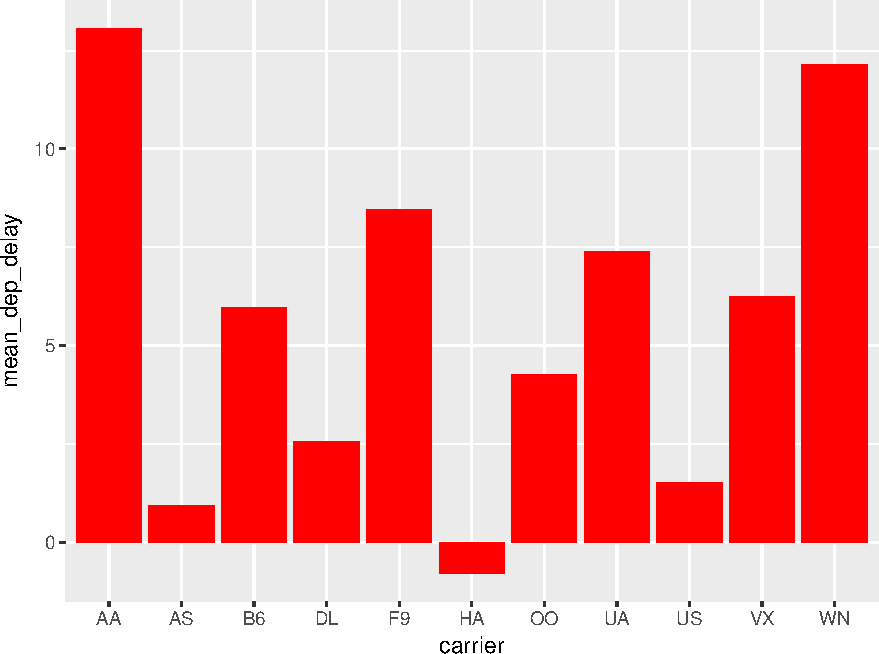
\includegraphics{thesis_files/figure-latex/delaysboxplot-1.pdf}
  \caption{\label{fig:delaysboxplot}Mean Delays by Airline}
  \end{figure}
  
  Here is a reference to this image: Figure \ref{fig:delaysboxplot}.
  
  A table linking these carrier codes to airline names is available at
  \url{https://github.com/ismayc/pnwflights14/blob/master/data/airlines.csv}.
  
  \clearpage
  
  Next, we will explore the use of the \texttt{out.extra} chunk option,
  which can be used to shrink or expand an image loaded from a file by
  specifying \texttt{"scale=\ "}. Here we use the mathematical graph
  stored in the ``subdivision.pdf'' file.
  
  \begin{figure}
  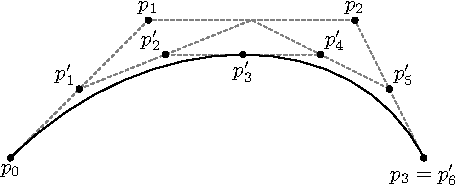
\includegraphics[scale=0.75]{figure/subdivision} \caption{Subdiv. graph}\label{fig:subd}
  \end{figure}
  
  Here is a reference to this image: Figure \ref{fig:subd}. Note that
  \texttt{echo=FALSE} is specified so that the \textbf{R} code is hidden
  in the document.
  
  \textbf{More Figure Stuff}
  
  Lastly, we will explore how to rotate and enlarge figures using the
  \texttt{out.extra} chunk option. (Currently this only works in the PDF
  version of the book.)
  
  \begin{figure}
  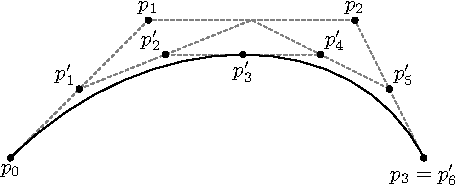
\includegraphics[angle=180, scale=1.1]{figure/subdivision} \caption{A Larger Figure, Flipped Upside Down}\label{fig:subd2}
  \end{figure}
  
  As another example, here is a reference: Figure \ref{fig:subd2}.
  
  \section{Footnotes and Endnotes}\label{footnotes-and-endnotes}
  
  You might want to footnote something.\footnote{footnote text} The
  footnote will be in a smaller font and placed appropriately. Endnotes
  work in much the same way. More information can be found about both on
  the CUS site or feel free to reach out to
  \href{mailto:data@reed.edu}{\nolinkurl{data@reed.edu}}.
  
  \section{Bibliographies}\label{bibliographies}
  
  Of course you will need to cite things, and you will probably accumulate
  an armful of sources. There are a variety of tools available for
  creating a bibliography database (stored with the .bib extension). In
  addition to BibTeX suggested below, you may want to consider using the
  free and easy-to-use tool called Zotero. The Reed librarians have
  created Zotero documentation at
  \url{http://libguides.reed.edu/citation/zotero}. In addition, a tutorial
  is available from Middlebury College at
  \url{http://sites.middlebury.edu/zoteromiddlebury/}.
  
  \emph{R Markdown} uses \emph{pandoc} (\url{http://pandoc.org/}) to build
  its bibliographies. One nice caveat of this is that you won't have to do
  a second compile to load in references as standard LaTeX requires. To
  cite references in your thesis (after creating your bibliography
  database), place the reference name inside square brackets and precede
  it by the ``at'' symbol. For example, here's a reference to a book about
  worrying: (Molina \& Borkovec, 1994). This \texttt{Molina1994} entry
  appears in a file called \texttt{thesis.bib} in the \texttt{bib} folder.
  This bibliography database file was created by a program called BibTeX.
  You can call this file something else if you like (look at the YAML
  header in the main .Rmd file) and, by default, is to placed in the
  \texttt{bib} folder.
  
  For more information about BibTeX and bibliographies, see our CUS site
  (\url{http://web.reed.edu/cis/help/latex/index.html})\footnote{Reed~College
    (2007)}. There are three pages on this topic: \emph{bibtex} (which
  talks about using BibTeX, at
  \url{http://web.reed.edu/cis/help/latex/bibtex.html}),
  \emph{bibtexstyles} (about how to find and use the bibliography style
  that best suits your needs, at
  \url{http://web.reed.edu/cis/help/latex/bibtexstyles.html}) and
  \emph{bibman} (which covers how to make and maintain a bibliography by
  hand, without BibTeX, at
  \url{http://web.reed.edu/cis/help/latex/bibman.html}). The last page
  will not be useful unless you have only a few sources.
  
  If you look at the YAML header at the top of the main .Rmd file you can
  see that we can specify the style of the bibliography by referencing the
  appropriate csl file. You can download a variety of different style
  files at \url{https://www.zotero.org/styles}. Make sure to download the
  file into the csl folder.
  
  \textbf{Tips for Bibliographies}
  
  \begin{itemize}
  \tightlist
  \item
    Like with thesis formatting, the sooner you start compiling your
    bibliography for something as large as thesis, the better. Typing in
    source after source is mind-numbing enough; do you really want to do
    it for hours on end in late April? Think of it as procrastination.
  \item
    The cite key (a citation's label) needs to be unique from the other
    entries.
  \item
    When you have more than one author or editor, you need to separate
    each author's name by the word ``and'' e.g.
    \texttt{Author\ =\ \{Noble,\ Sam\ and\ Youngberg,\ Jessica\},}.
  \item
    Bibliographies made using BibTeX (whether manually or using a manager)
    accept LaTeX markup, so you can italicize and add symbols as
    necessary.
  \item
    To force capitalization in an article title or where all lowercase is
    generally used, bracket the capital letter in curly braces.
  \item
    You can add a Reed Thesis citation\footnote{Noble (2002)} option. The
    best way to do this is to use the phdthesis type of citation, and use
    the optional ``type'' field to enter ``Reed thesis'' or
    ``Undergraduate thesis.''
  \end{itemize}
  
  \section{Anything else?}\label{anything-else}
  
  If you'd like to see examples of other things in this template, please
  contact the Data @ Reed team (email
  \href{mailto:data@reed.edu}{\nolinkurl{data@reed.edu}}) with your
  suggestions. We love to see people using \emph{R Markdown} for their
  theses, and are happy to help.
  
  \chapter*{Conclusion}\label{conclusion}
  \addcontentsline{toc}{chapter}{Conclusion}
  
  \chapter{The First Appendix}\label{the-first-appendix}
  
  \chapter*{References}\label{references}
  \addcontentsline{toc}{chapter}{References}
  
  \hypertarget{refs}{}
  \hypertarget{ref-alexander2009}{}
  Alexander, D. (2009). \emph{Fast model-based estimation of ancestry in
  unrelated individuals.}
  
  \hypertarget{ref-caye2016}{}
  Caye, K. (2016). \emph{TESS3: Fast inference of spatial population
  structure and genome scans for selection.}
  
  \hypertarget{ref-frichot2015}{}
  Frichot, É. (2015). \emph{LEA: An r package for landscape and ecological
  association studies.}
  
  \hypertarget{ref-harrison1990hybrid}{}
  Harrison, R. G., \& others. (1990). Hybrid zones: Windows on
  evolutionary process. \emph{Oxford Surveys in Evolutionary Biology},
  \emph{7}, 69--128.
  
  \hypertarget{ref-maples2013}{}
  Maples, B. K. (2013). \emph{RFMix: A discriminative modeling approach
  for rapid and robust local-ancestry inference.}
  
  \hypertarget{ref-mcvean2009}{}
  McVean, G. (2009). A genealogical interpretation of principal components
  analysis.
  
  \hypertarget{ref-Molina1994}{}
  Molina, S. T., \& Borkovec, T. D. (1994). The Penn State worry
  questionnaire: Psychometric properties and associated characteristics.
  In G. C. L. Davey \& F. Tallis (Eds.), \emph{Worrying: Perspectives on
  theory, assessment and treatment} (pp. 265--283). New York: Wiley.
  
  \hypertarget{ref-noble2002}{}
  Noble, S. G. (2002). \emph{Turning images into simple line-art}
  (Undergraduate thesis). Reed College.
  
  \hypertarget{ref-price2009}{}
  Price, A. L. (2009). \emph{Sensitive detection of chromosomal segments
  of distinct ancestry in admixed populations.}
  
  \hypertarget{ref-reedweb2007}{}
  Reed~College. (2007, march). LaTeX your document. Retrieved from
  \url{http://web.reed.edu/cis/help/LaTeX/index.html}
  
  \hypertarget{ref-suarez2016}{}
  Suarez-Gonzalez, et a., Adriana. (2016). Genomic and functional
  approaches reveal a case of adaptive introgression from populus
  balsamifera (balsam poplar) in p. trichocarpa (black cottonwood).
  \emph{Molecular Ecology}, 2427--2442.
  
  \hypertarget{ref-thornton2014}{}
  Thornton, T. (2014). \emph{Local and global ancestry inference, and
  applications to genetic association analysis for admixed populations.}
  
  \hypertarget{ref-yang2013}{}
  Yang, J. J. (2013). \emph{Efficient inference of local ancestry.}


  % Index?

\end{document}

